\section{Methodologie}
\label{sec:meth}


\subsection{De data}
De data die gebruikt worden, zijn de Handelingen van de Tweede Kamer gedurende het missionaire kabinet-Rutte II (5 november 2012 tot 22 maart 2017). Er is gekozen voor dit kabinet, omdat de data hiervoor makkelijk verkrijgbaar was, het kabinet lang zat, waardoor er veel data is, en het recent is waardoor het makkelijker te interpreteren is. Deze data zijn in xml-formaat van de website officielebekendmakingen.nl gehaald, samen met corresponderende metadata xml-bestanden. De bestanden van de Handelingen bevatten voornamelijk informatie over spreekbeurten tijdens een debat, waaronder naam van een spreker, partij-affiliatie, inhoud van de spreekbeurt en het soort spreekbeurt. Deze gegevens zijn samengevoegd tot een tabel en opgeslagen als csv-bestand.\par
Deze dataset bestaat uit een aantal soorten spreekbeurten; debat bijdragen, interrupties en antwoorden. Debat bijdrage is de eerste onafgebroken spreekbeurt die een spreker geeft achter het spreekgestoelte, aangeduid in de xml-file met het attribuut \textit{nieuw="ja"}. Dit kan een bijdrage in een debat zijn of een vraag tijdens een vragenuur. Interrupties zijn de vragen die andere politici stellen vanachter de interruptiemicrofoon aan de spreker. De antwoorden zijn vervolgens de reactie van een spreker achter het spreekgestoelte op een interruptie. Aangezien een debat bijdrage geïnterrumpeerd kan worden, kan deze inhoudelijk doorlopen in een antwoord van een spreker. Er is in dit onderzoek ervoor gekozen om gebruik te maken van een debat bijdrage samengevoegd tot één document met alle bijbehorende antwoorden van die spreker. Daarnaast zijn er verschillende soorten sprekers; de voorzitter, Tweede Kamerleden, leden van het kabinet en gastsprekers.  Daarnaast is alleen gekozen voor sprekers waarvan er een partij-affiliatie vermeld staat, dit is niet het geval voor leden van het kabinet, de voorzitter en gastsprekers  (met uitzondering van Nederlandse leden van het Europees Parlement).\par
Deze dataset bevat vervolgens naast de verkozen partijen van de 2012 Tweede Kamerverkiezingen, ook afsplitsingen van die partijen (tien in totaal) en bezoeken van vertegenwoordigingen van Nederlandse partijen uit het Europees Parlement (tien in totaal). Omdat van beide categorieën relatief weinig data is en er overlap zit met hun oorspronkelijke partij, zijn deze er uit gehaald. Op basis van de aantallen is er voor classificatie een baseline nauwkeurigheid van 0.15 (door altijd grootste partij te kiezen) en baseline $F_1$ score van 0.11 (door willekeurig te voorspellen gewogen bij aantal spreekbeurten in klasse).\par

De documenten verschillen vervolgens in grootte. De distributie lijkt op een lognormale verdeling, maar met een Kolmogorov-Smirnov test is hier geen bewijs voor gevonden \cite{Scipy}.

\begin{figure}%
    \centering
    \subfloat[label 1]{{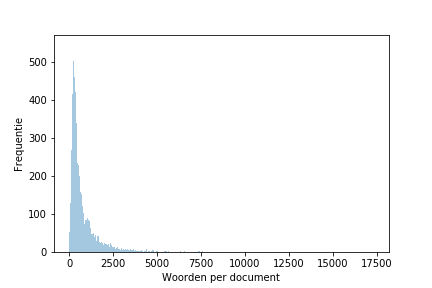
\includegraphics[width=5cm]{Verslag/Tables/lengthtexts.png} }}%
    \qquad
    \subfloat[label 2]{{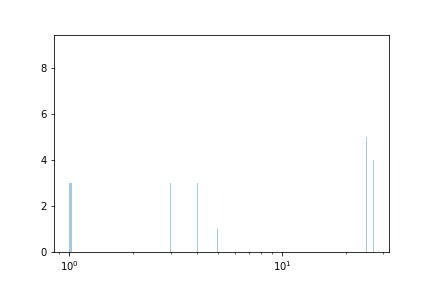
\includegraphics[width=5cm]{Verslag/Tables/lengthtextslog.png} }}%
    \caption{2 Figures side by side}%
    \label{fig:example}%
\end{figure}



\subsection{Methoden}


\subsubsection{Deelvraag 1}
Om deze deelvraag te beantwoorden zullen een aantal classificatiemethoden vergeleken worden. Aangezien het onmogelijk is om alle classificatiemethoden te vergelijken, beperkt dit onderzoek zich tot classificatiemethoden die gebruikt zijn in vergelijkbare onderzoeken, zoals besproken in \ref{sec:Deelvraag1}. Er is ervoor gekozen om alleen gebruik te maken van methoden waarvan reeds implementaties beschikbaar waren in Python. Hieronder worden de verschillende onderdelen besproken.

\paragraph{Pre-processing}
Voor pre-processing is gebruik gemaakt van tokenisation en lowercasing. Voor tokenisation is de reguliere expressie $\\w+$ gebruikt, die daarmee alleen de letters en cijfers overhoudt. Deze woorden zijn vervolgens allemaal omgezet in kleine letters. Vervolgens is er gevarieerd tussen wel of geen gebruik maken van stemming. In het geval van stemming is gebruik gemaakt van de Snowball Stemmer via de Python NLTK module.

\paragraph{Bag-of-words model}
Bag-of-words model is de meest gebruikte representatie van data in vergelijkbare onderzoeken. Bij het bag-of-words model wordt elk document gerepresenteerd door een vector, waarbij elke kolom een woord voorstelt met een bijbehorende waarde. Voornaamste beperking van dit model is dat het geen rekening houdt met de volgorde van woorden, wat een groot effect kan hebben op de betekenis van een document.\par
Voor dit onderzoek zijn de volgende wegingen voor woorden getest: \textit{boolean} (wel of niet aanwezig), \textit{tf} (woordfrequentie), \textit{tf-norm} (woordfrequentie genormaliseerd door documentlengte) en \textit{tf-idf}
Daarnaast wordt in dit onderzoek geëxperimenteerd met een minimale of maximale woord- of documentfrequentie. Ook is gekeken naar het effect van combinaties van unigrams, bigrams en trigrams.\par

\paragraph{Support Vector Machines en Logistische Regressie}
De meest voorkomende techniek in vergelijkbaar onderzoek is Support Vector Machine (SVM). Een andere techniek die gebruikt wordt is logistische regressie. Beide kennen een eigen implementatie in sklearn, maar gezien de grootte van de dataset, duurt dit te lang met een gridsearch. Om deze reden is er in beide gevallen voor gekozen om gebruik te maken van de functie SGDClassifier, die beide technieken leert met \textit{stochastic gradient descent learning}. Er is hiervoor gevarieerd met de regularisatie, learning rate en maximum aantal iteraties. Voor regularisatie is hier geëxperimenteerd met Lasso en Ridge regularisatie, en een combinatie van beide genaamd Elasticnet. De andere parameters zijn gelaten op de standaardwaarden van scikit-learn.\cite{scikit-learn}.\par
% https://towardsdatascience.com/how-to-make-sgd-classifier-perform-as-well-as-logistic-regression-using-parfit-cc10bca2d3c4

\paragraph{Naive Bayes}
Een simpelere techniek die gebruikt wordt voor politieke tekstclassificatie is Naive Bayes. Dit algoritme neemt aan dat elke \textit{feature} onafhankelijk is ten op zichte van de rest. Dit is bij tekstclassificatie vaak niet het geval omdat het gebruik van sommige woorden gepaard kan gaan met het gebruik van andere woorden. Daarnaast is het gebruik van meerdere n-grams in een classificatie schending van de aanname, want als bijvoorbeeld een bigram er in voorkomt dan komen ook beide unigrams er sowieso in voor. Desalniettemin blijkt Naive Bayes effectief te zijn voor tekstclassificatie\cite{scikit-learn,bhand}. Hiervoor zijn de functies van scikit-learn MultinomialNB en BernoulliNB gebruikt.\cite{scikit-learn,bhand}\par

\paragraph{Beoordelen van kwaliteit}
De meest gebruikte methoden om kwaliteit van politieke tekstclassificatie te beoordelen zijn accuracy en $F_1$ score, die opgebouwd is uit recall en precision. Deze scores zijn opgebouwd uit het aantal correct positief ($tp$), foutief positief ($fp$), correct negatief ($tn$) en foutief negatief ($fn$) geclassificeerde waarden.\par
\begin{equation}
    Precision = \frac{tp}{tp + fp}\\
\end{equation}
\begin{equation}
    Recall = \frac{tp}{tp + tn}
\end{equation}
\begin{equation}
    Accuracy = \frac{tp + tn}{tp + tn + fp + fn}
\end{equation}
\begin{equation}
    F_1 = 2 * \frac{Precision * Recall}{Precision + Recall}
\end{equation}
Deze waarden worden per klasse bepaald en daar wordt vervolgens een gemiddelde van genomen, gewogen bij documenten behorende tot die klasse.  \cite{Manning:2008:IIR:1394399,scikit-learn}.\par
% https://nlp.stanford.edu/IR-book/html/htmledition/evaluation-of-text-classification-1.html
\bigskip
Voor de classificatiemethoden wordt waar mogelijk gebruik gemaakt van functies van de Python module scikit-learn\cite{scikit-learn}, aangevuld met zelf geschreven code als dit niet reeds beschikbaar is. Bij al deze classificatiemethoden wordt gevarieerd met meerdere parameters door middel van een gridsearch. Hierbij wordt gebruikt gemaakt van 5-fold cross-validation. Daardoor wordt de data gespleten in vijf delen, waarvan steeds één deel als testset wordt gebruikt en de rest voor training.

\subsubsection{Deelvraag 2}
In het onderzoek van Diermeier et al. worden alle eigennamen weggelaten zodat, volgens hen, namen van personen en partijen niet de classificatie domineren. Aangezien hier bij deelvraag 1 niet voor is gekozen, wordt bij deze deelvraag gekeken hoe groot het effect hiervan is, specifiek gericht op partijnamen en achternamen van kamerleden. Voor deze deelvraag wordt wederom een classificatie gedaan met de classificatiemethode die resulteerde uit deelvraag 1. In deze classificatie worden alle partijnamen vervangen door de tag PARTIJNAAM en alle namen van Kamerleden vervangen door de KAMERLIDNAAM. Deze namen zijn uit de Handelingen gehaald. Voor partijnamen zijn ook lidwoorden toegevoegd, voor achternamen van kamerleden zijn ook verkortingen meegenomen. Dit laatste omdat bijvoorbeeld \textit{Van Haersma Buma} vaak aangesproken wordt als \textit{Buma}. Voornamen van Kamerleden worden zelden tot nooit gebruikt, dus die zijn er niet uitgehaald. Een nadeel van deze aanpak is dat ook namen van niet-kamerleden of andere woorden weggehaald kunnen worden als deze hetzelfde zijn als naam van een kamerlid. Door gebruik van gevoeligdheid voor hoofdletters is geprobeerd dit te voorkomen. Een opvallend voorbeeld hiervan is de naam Rutte, die zowel behoort tot het kamerlid Arno Rutte als de premier Mark Rutte.\par
De nauwkeurigheid en $F_1$ score worden vervolgens vergeleken met de resultaten uit deelvraag 1. Ook wordt gekeken naar verschillen tussen de meest veelzeggende woorden uit deelvraag 1 en uit deze deelvraag.

\subsubsection{Deelvraag 3}

Om deze deelvraag te beantwoorden zullen de twee experimenten die Graeme Hirst et al. uitvoerden voor dezelfde vraag gereproduceerd worden op de dataset van de Tweede Kamer. Bij deze deelvraag zal de beste classifier uit deelvraag 1 gebruikt worden. Daarnaast kan men ook naar de confusion matrix kijken of het aantal verkeerde classificaties groter is binnen regering of oppositie dan tussen elkaar.\par
In het eerste experiment zullen de tien meest karakteristieke woorden per partij van de ene zittingsperiode vergeleken worden met de tien meest karakteristieke woorden per partij van de andere zittingsperiode. Als de classificatie op basis van ideologie is in plaats van partij-status, is het te verwachten dat de woorden bij een partij blijven en niet gekoppeld zijn aan in oppositie of regering zitten. \par
In het tweede experiment worden classifiers getraind op de ene zittingsperiode en getest op de andere zittingsperiode. Als de classificatie op basis van ideologie is in plaats van partij-status, is de verwachting dat er nog steeds aanzienlijke voorspellingen gedaan worden, aangezien de ideologie naar verwachting redelijk stabiel is binnen tien jaar (hoewel woordgebruik varieert). Als de scores aanzienlijk lager zijn, kan dit het gevolg zijn van het veranderen van partij-status van partijen.\par
Als vergelijkingsmateriaal is voor deze experimenten een tweede dataset nodig uit een ander kabinet. Hiervoor is het wenselijk dat dit kabinet bestaat uit andere partijen dan kabinet-Rutte II. Daarnaast is het ook wenselijk als het niet te ver terug is, zodat onderwerpen en taalgebruik enigszins overeenkomstig zijn. Omdat kabinet-Rutte I een minderheidskabinet was met een bijzondere partij-status voor de PVV, is ervoor gekozen om de Handelingen van de Tweede Kamer tijdens het missionaire kabinet-Balkenende IV (22 februari 2007 tot 20 februari 2010) te gebruiken.\par

\subsubsection{Deelvraag 4}
Voor deze deelvraag vergelijken we de resultaten van de eerdere classificatie per partij met een binaire classificatie op basis van rechts en links. Hiervoor wordt wederom de dataset van kabinet-Rutte 2 gebruikt, met het model wat resulteerde uit deelvraag 1. \par
Voor deze vraag moet vastgesteld worden welke partijen links en rechts zijn. Omdat dit lastig te bepalen is en er meerdere indelingen zijn, wordt hier gebruik gemaakt van twee verschillende indelingen. De indeling op basis van het Kieskompas van Andre Krouwel voor de Kamerverkiezing 2012 en de indeling volgens het Manifesto Project\cite{Volkens:2017} gebaseerd op verkiezingsprogramma's voor de Kamerverkiezing van 2012. In beide gevallen is de nullijn van het politieke spectrum gebruikt om te bepalen of een partij links of rechts is.\par

\begin{table}[H]
\centering
\caption{Rechts (R) of link (L) indeling per partij op basis van het Kieskompas en het Manifesto Project.}
\label{my-label}
\centering
\begin{tabular}{lll}
\hline
Partij  & Kieskompas & Manifesto Project \\ \hline
SP           & L & L\\ 
PvdA         & L & L\\ 
GroenLinks   & L & L\\ 
PvdD         & L & L\\ 
50PLUS       & L & L\\ 
D66          & R & L\\ 
PVV          & - & R\\ 
ChristenUnie & R & R\\ 
SGP          & R & R\\ 
VVD          & R & R\\ 
CDA          & R & R\\
\end{tabular}
\end{table}

% hypothese

% https://www.google.nl/search?q=grafiek+2012+kieskompas&safe=off&source=lnms&tbm=isch&sa=X&ved=2ahUKEwjigpaDoIXbAhUSJlAKHUBzBQ4Q_AUoAXoECAAQAw&biw=1920&bih=943#imgrc=Dekv0sSQBTnikM: